\documentclass[tikz, border=2pt]{standalone}
\usepackage{tikz}
\usepackage{pgfplots}
\usetikzlibrary{decorations.pathreplacing,calc}
\begin{document}
    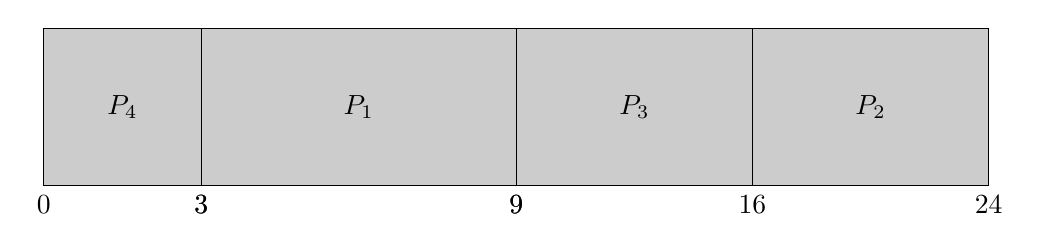
\begin{tikzpicture}
        \draw [fill=black!20] (0,0) rectangle (2,2) 
            node [midway] {$P_4$} 
            node [pos=0, below] {0}
            node at (2,0) [below] {3};
        \draw [fill=black!20] (2,0) rectangle (6,2) 
            node [midway] {$P_1$}
            node [pos=0, below] {3}
            node at (6,0) [below] {9};
        \draw [fill=black!20] (6,0) rectangle (9,2) 
            node [midway] {$P_3$}
            node [pos=0, below] {9}
            node at (9,0) [below] {16};
        \draw [fill=black!20] (9,0) rectangle (12,2)
            node [midway] {$P_2$}
            node at (12,0) [below] {24};
    \end{tikzpicture}
\end{document}